\chapter{Makahiki and SGSEAM Evaluation}
\label{cha:evaluation}

This chapter describes the way I evaluated the Makahiki framework described in \autoref{cha:system-description} and the SGSEAM method described in \autoref{cha:framework-description}. First, I describe the Real-world case studies of Makahiki instances realized in the Kukui Cup Challenges at the different organizations, followed by the detailed assessment of applying SGSEAM to Makahiki framework. The evaluation is to address:
(a) obtain insights about the strength and weakness of the Makahiki serious game framework, (b) obtain insights about the strength and weakness of SGSEAM serious game framework assessment method.

\section{Real-world Makahiki Instances Case Studies}

Makahiki, as a serious game framework for sustainability, had been used by different organizations to create multiple serious game instances targeting to educate and foster sustainable behavior among the communities. The first Kukui Cup Energy challenges at the University of Hawaii at Manoa (UHM) were held in 2011 for 3 weeks for over 1,000 first year students living in the residence halls. UHM subsequently held the second and third Kukui Cup Energy challenges in 2012 and 2014 for different first year students and different durations, for 9 months and 2 weeks respectively. Hawaii Pacific University (HPU) held their Kukui Cup Energy challenge in Fall 2012 and 2013 for about 200 students each year. An international organization called the East-West Center (EWC) held a Kukui Cup Energy and Water challenge for the international residents living in the residenct halls. An Hawaii private school called Holy Nativity School (HNS) held a pilot Kukui Cup challenge for the middle school students. 

Table \autoref{table:instances} lists these instances and their different requirements. The major requirements are differed in the duration of the challenge, population that could participate in the challenge, the type of resource such as energy or water, whether they have smarter meters installed, and type of web server hosting. Additional difference in requirements includes the type of the authentication for the participation, the differences in the game mechanics implementation. These differences will be described in the result chapter in more details.

\begin{table}[ht!]
  \centering
  \begin{tabular}{|p{0.15\columnwidth}|p{0.15\columnwidth}|p{0.15\columnwidth}|p{0.15\columnwidth}|p{0.15\columnwidth}|p{0.15\columnwidth}|}
    \hline
    \tabhead{Instances} &
    \tabhead{Duration} &
    \tabhead{Populations} &
    \tabhead{Resource} &
    \tabhead{Smart meters} &
    \tabhead{Hosting} \\
    \hline
    UHM 2011 & 3 weeks & 1038 & Energy & Yes & Local \\
    \hline
    UHM 2012 & 9 months & 1067 & Energy & Yes & Cloud \\
    \hline
    UHM 2014 & 2 weeks & 1056 & Energy & Yes & Cloud \\
    \hline
    HPU 2012 & 3 weeks & 198 & Energy & Yes & Local \\
    \hline
    HPU 2013 & 3 weeks & 197 & Energy & Yes & Local \\
    \hline
    EWC 2012 & 2 weeks & 129 & Energy and Water & No & Cloud \\
    \hline
    HNS 2013 & 4 weeks & 10 & Energy & Yes(simulated) & Cloud \\
    \hline    
  \end{tabular}
  \caption{Makahiki Serious Game Instances}
  \label{table:instances}
\end{table}

The Makahiki instances deployed at these organizations have to meet these different requirements. The goal of the Makahiki framework is to minimize the effort in supporting the different requirements in various organizations. The case study evaluation approach of Makahiki is to look at the different requirements of these organizations, and the corresponding different configurations in the Makahiki framework to support such requirements. A more formal assessment of the strength and weakness of the Makahiki framework is described in the next section, by applying SGSEAM to Makahiki, which assessing the experiences of various stakeholders of the Makahiki framework.

\section{Applying SGSEAM to Makahiki}

This section describes in details the application of SGSEAM to assess the Makahiki framework in order to identified the strengths and weaknesses of both the Makahiki and the SGSEAM itself.

\subsection{SGSEAM Stakeholders in Makahiki}
The first step in SGSEAM assessment method is to identify the stakeholders in Makahiki. \autoref{table:stakeholders} listed the identified stakeholders who use the Makahiki framework. 

\begin{table}[ht!]
  \centering
  \begin{tabular}{|p{0.2\columnwidth}|p{0.4\columnwidth}|p{0.3\columnwidth}|}
    \hline
    \tabhead{Stakeholder class} &
    \tabhead{Tasks} &
    \tabhead{Role} \\
    \hline
    Player &
    Participate in the Makahiki games &
    Students living in the residential halls\\
    \hline
    System admin &
    Install Makahiki software, minitor and scale the system, backup, patch maintenance &
    IT staffs\\
    \hline
    Game designer &
    Design the content, configure suitable games and mechanics &
    Challenge organizers\\
    \hline
    Game manager &
    Manage the game during the period of game play.&
    Challenge organizers\\
    \hline
    Game developer &
    Develop customization, extend and enhance the game and framework. &
    Makahiki developers \\
    \hline
  \end{tabular}
  \caption{SGSEAM Stakeholders}
  \label{table:stakeholders}
\end{table}

\subsection {SGSEAM Approach for Makahiki}

The second step in SGSEAM is to determine the assessment approach. As described in SGSEAM, The assessment approaches is categorized into in-vivo and in-vitro assessments. The in-vivo approaches, such as pre-post test, in-game surveys and post-hoc interviews, assess the real world instance of the game. The in-vitro approaches use in-lab experiments in a simulated environment. Different assessment approaches will have different levels of rigor or validity. When applying SGSEAM in Makahiki, I used the real world Makahiki instances as the in-vivo approaches which includes pre-post effectiveness study for player assessment, post-hoc interview for game administrator and game designer. 

In addition to real world instances assessment, I also implemented the in-vitro assessment approach using the in-lab experiments. In Spring 2012, Professor Philip Johnson at the Information and Computer Science Department of University of Hawaii used Makahiki to teach a course in serious game development. The students were seniors or graduate students majoring in computer science related fields. During the course, the students installed Makahiki, designed a serious game instance with Makahiki, and developed an enhancement to the Makahiki system.

Besides the real world usage of Makahiki in the series of Kukui Cup challenges, we
performed in-lab assessment experiments in 2013. Makahiki was used in a serious game
development course in Spring semester of 2013 at the Information and Computer Sciences
Department of the University of Hawaii at Manoa. There were a total of 8 students who
participated in the experiments.  The participants were either senior undergraduates or
graduate students majoring in Computer Science. During the course, the students installed
Makahiki, configured and designed a serious game instance with Makahiki, and finally
developed an enhancement to the Makahiki framework. We asked the students taking the
course to voluntarily participate in the assessment experiments of Makahiki, using SGSEAM.

These students participated in the assessment experiments of Makahiki, in the aspects of system admin efficiency, game designer efficiency and developer efficiency. The participation is voluntary. This is considered as an in-lab experiment since they are evaluating Makahiki in a class setting and using Makahiki in the development environments.

\autoref{table:approaches} lists the SGSEAM approaches that are used to assess the strengths and weaknesses of Makahiki from different stakeholders' view.

\begin{table}[ht!]
  \centering
  \begin{tabular}{|p{0.175\columnwidth}|p{0.3\columnwidth}|p{0.43\columnwidth}|}
    \hline
    \tabhead{Stakeholder}&
    \tabhead{Assessment approaches} &
    \tabhead{Expected Outcomes} \\
    \hline
    {\multirow{3}{*}{Player}}&
    Pre-post effectiveness study(\ref{Pre-Post effectiveness study}) &
    Determine effectiveness in energy literacy and resource usage reduction \\
    \cline{2-3}
    {}&
    Self-reported usability metrics(\ref{Self-reported usability metrics}) &
	Identify problem areas in game interface\\
    \cline{2-3}
    {}&
	Engagement metrics(\ref{Engagement metrics}) &
	Determine the extent of engagement\\
    \hline
    {\multirow{2}{*}{System admin}}&
    Post-hoc admin interview(\ref{Post-hoc system admin interview}) &
    {\multirow{2}{*}{Determine strengths and weaknesses in system install and maintenance}}\\
    \cline{2-3}
    {}&
    In-lab system admin study(\ref{In-lab system admin study}) &
    {}\\
    \hline
    Game designer&
    Determine strengths and weaknesses in facilitating the game design process.&
    	Post-hoc designer interview(\ref{Post-hoc game designer interview});\newline
	Game design log data analysis(\ref{Game design log data analysis});\newline
	In-lab game design study(\ref{In-lab game design study})\\
    \hline
    Game manager&
    Determine strengths and weaknesses in managing the game.&
    	Post-hoc manager interview(\ref{Post-hoc game manager interview});\newline
	Game management log data analysis(\ref{Game management log data analysis});\newline
	In-lab game management study(\ref{In-lab game management study})\\
    \hline
    Game developer&
    Determine strengths and weaknesses in developing system enhancement.&
    	Post-hoc developer interview(\ref{Post-hoc game developer interview});\newline
	In-lab game development study(\ref{In-lab game development study}) \\
    \hline
  \end{tabular}
  \caption{SGSEAM approaches}
  \label{table:approaches}
\end{table}

The following sections describe the assessment approaches in details. 

\subsubsection{Player assessment}

I applied the SGSEAM player assessment mechanism to the 2011 real-world Kukui Cup instance at the University of Hawaii at Manoa to study the player's experience with the Makahiki framework. There are over 1000 eligible players for this instances. They are the first year college student living in four similar structured resident halls in close vicinity. The challenge lasted for 3 weeks. Makahiki system recorded the logging data from every interaction between the players and the website.

To assess the effectiveness of the framework for designing games that improve player literacy in sustainability, we
conducted two energy literacy surveys, one before the challenge (pre-game) and one after
the challenge (post-game). SurveyGizimo is used to create the surveys which consists of the set of sustainability literacy and behavior questionnaires. The response from the two surveys are analyzed to provide insights about the player's literacy and behavior change.

To assess the effectiveness of the framework for designing games that produce positive change in sustainability
behaviors, we recorded and analyzed energy consumption data before, during and after the
challenge.  Before the challenge, an energy usage baseline was established. The energy consumption data is examined to understand any usage pattern or reduction during and after the challenge.

To assess the usability of the game produced by the Makahiki framework, we conducted the in-game usability survey. The survey asked the questions about the players' experience about the user interface of the game. The response from the survey is analyzed to provide insights about the game usability.

In addition to the surveys and energy data measurement, the following engagement metrics is calculated based on the log data to assess the engagement level of the instance:

\begin{itemize}
\item active participation rate
\item number of players per day
\item average session time
\item submissions per day
\item level of social engagement
\item website errors
\end{itemize}

\subsubsection{System admin assessment}

There are two approaches described in SGSEAM to assess the system admin's experience: One is the in-lab experiments, another is the interview of the system admin of a real world instance.

In the in-lab experiments, the students in the ICS691 Spring 2013 class were tasked with installing the Makahiki system into their local computers as well as the cloud environment. In order to understand how much time it takes to install the Makahiki and what problems might be encountered, I design a Google form which details the steps of installing Makahiki both locally and in the cloud, and for each step, I ask the students to record the time they spent and the problems they encountered.

Figure \ref{fig:developer-eval-form} illustrates a partial google form used for Makahiki system admin assessment. \autoref{app:googleform} includes the complete google form.
\begin{figure}[ht!]
   \centering
   \includegraphics[height=30em,width=30em]{developer-eval-form.eps}
   \caption{Makahiki Developer assessment Form}
   \label{fig:developer-eval-form}
\end{figure}

The students were also asked to provide feedback about their installation experiences in the form of blog post. In the blog post, I ask them to discuss the following topics:
\begin{itemize}
\item What is the most difficult step during installation?
\item What problems did you encounter during the installation?
\item Have you install any database, web server or similar server products prior to this assignment? Are those installations for development or production purpose?
\item If you have experience installing other servers before, How does your prior experience of installing other servers compare to the installation of Makahiki?
\item What could be improved about the Makahiki installation process?
\item Compare your experience of installing Makahiki in Heroku with installing it locally,
\end{itemize}

The qualitative data collected from the google form response and the blog post from the students will be analyzed to gain insights into how easy it is to install Makahiki, and what contributes to the efficiency of the installation.

In order to gain insights on the experience of a real world system admin who uses the Makahiki, I performed interviews to the system admins of the 2012 Hawaii Pacific University (HPU) challenges.

I analyzed qualitative data collected from the interviews and email changes. The data include:
\begin{itemize}
 \item time taken to install the Makahiki
 \item time taken to maintain the Makahiki, such as backup, monitoring
 \item problems encountered
\end{itemize}

\subsubsection{Game designer assessment}

There are also two approaches described in SGSEAM to assess the game designer's experience: One is the in-lab experiments, another is the interview of the game designer of a real world instance.

The students in the in-lab experiments were tasked to design a Kukui Cup like serious game using Makahiki. I designed another google form to ask students to follow the designing steps and record their time and problem encountered during their designing process. \autoref{app:googleform} has the complete google form for the steps the students need to follow.

The students were asked to provide feedback about their installation experiences in the form of blog post to discuss the following topics:
\begin{itemize}
\item What is the most difficult step during Challenge Design?
\item What problems did you encounter while designed the challenge?
\item What problems did you encounter while managing the challenge?
\item What could be improved for the Makahiki Challenge Design process?
\item What could be improved for the Makahiki Challenge Management process?
\end{itemize}

I performed interviews to the real world game designers of the 2012 Hawaii Pacific University challenges. We asked him about his game designing experiences using the Makahiki admin
 interface.

I analyzed both the qualitative data collected from the interviews and email changes with the game designers, and the quantitative collected from the admin interface log data. The qualitative data includes:
\begin{itemize}
    \item How much time did you spend to configure the challenge global settings?
    \item how much time did you spend to setup the player data?
    \item how much time did you spend to design the individual games?
    \item What problem did you encountered?
    \item Did you find it difficult to configure? what is difficult?
    \item Did you find it difficult to design a specific game? which one, what is difficult?
    \item What did you like the least when using the system?
\end{itemize}

The quantitative data includes:
\begin{itemize}
 \item time taken to configure the challenge with regarding to different designing tasks
 \item problems encountered in the log file
\end{itemize}

\subsubsection{Game manager assessment}
I performed interviews to the real world game managers of the 2012 Hawaii Pacific University challenges to study the experience of the game management using Makahiki.

I analyzed both the qualitative data collected from the interviews and email changes with the game managers, and the quantitative collected from the admin interface log data. The qualitative data includes:
\begin{itemize}
\item How much time did you spend to approving the action submissions?
\item How much time did you spend to monitoring the game status?
\item How much time did you spend to notifying prize winners?
\item What problem did you encountered?
\item Did you find it difficult to manage? what is difficult?
\item What did you like the least when using the system?
\end{itemize}

The quantitative data include:
\begin{itemize}
 \item time taken to manage the challenge with regarding to different managing tasks
 \item problems encountered in the log file
\end{itemize}

\subsubsection{Developer assessment}

The students in the in-lab experiment are tasked with developing an enhancement to the Makahiki instance. This involves setting up the development environment, following the tutorial to create the "Hello world" widget using Makahiki, and finally, develop the enhancement which extends the functionality of the Makahiki system.

The students are asked to submit their development source code to the public source code repository (Github) and write a blog post to discuss their efforts to complete the development activity.

I reviewed their source code to compare their code to the reference implementation, analyze the blog post from the students, as well as any email correspondence from students discussing  problems during the development.

\subsection{Assessment Participants}

After the assessment approaches are determined, the next step in SGSEAM is to identify the assessment participants for the different stakeholders. Table \autoref{table:participants} lists the participants for assessing the Makahiki framework using SGSEAM. 

\begin{table}[ht!]
  \centering
  \begin{tabular}{|p{0.2\columnwidth}|p{0.4\columnwidth}|p{0.3\columnwidth}|}
    \hline
    \tabhead{Stakeholder class} &
    \tabhead{Person(s)} &
    \tabhead{Organization} \\
    \hline
    Player &
    All eligible players in the UH KC 2011 instance &
    University of Hawaii at Manoa\\
    \hline
    System admin &
    ICS691 students for in-lab experiment, system admin for HPU 2012 instance &
    University of Hawaii at Manoa, Hawaii Pacific University\\
    \hline
    Game designer &
    ICS691 students for in-lab experiment, game designer for HPU 2012 instance &
    University of Hawaii at Manoa, Hawaii Pacific University\\
    \hline
    Game manager &
    ICS691 students for in-lab experiment, game designer for HPU 2012 instance &
    University of Hawaii at Manoa, Hawaii Pacific University\\
    \hline
    Game developer &
    ICS691 students for in-lab experiment &
    University of Hawaii at Manoa \\
    \hline
  \end{tabular}
  \caption{SGSEAM Stakeholders}
  \label{table:participants}
\end{table}

\subsection{Assessment Data Collection and Analysis}

The SGSEAM assessment process for Makahiki is carried out by implementing the different assessment approaches for the stakeholder participants, both in real world Makahiki instances and in-lab experiments. The data collected from all the different assessment approaches includes:

\begin{itemize}
\item pre-post surveys from players
\item in-game usability survey from players
\item interviews audio recordings from system admin, game designers, game managers
\item email communications from system admin, game designers, game managers
\item website logs and errors
\item google forms results reported from in-lab experiment evaluation
\end{itemize}

The data is analyzed according to the assessment approach to determine the strengths and weaknesses of the Makahiki framework with the respects of the different stakeholders in questions.